\RequirePackage{fix-cm}
\documentclass[twocolumn]{svjour3}          % twocolumn
%
\smartqed  % flush right qed marks, e.g. at end of proof
%
\usepackage{graphicx}
\usepackage{xeCJK}
\setCJKmainfont{BabelStone Han}

\begin{document}

\title{一种规范的实现敏捷开发实践的方法:敏捷开发框架}

\author{Ahmed Sidky \and James Arthur \and Shawn Bohner}

\institute{S. Bohner \at  Virginia Tech, Blacksburg, VA, USA \\ \email{sbohner@vt.edu} \and
           A. Sidky \at \email{asidky@vt.edu} \and
           J. Arthur \at \email{arthur@vt.edu}
}

\date{Received: 6 March 2007 / Accepted: 8 May 2007 / Published online: 24 July 2007}

\maketitle

\begin{abstract}
很多公司期望应用敏捷开发来利用它所带来的多种优势。这些优势包括更快的投资回报率、更高的软件质量和更高的客户满意度,当然其带来的好处不仅仅是局限于此。然而,到目前为止没有一种结构化的处理方式来指导公司如何实践敏捷开发。为了解决这个问题,我们提出了一种敏捷应用框架和我们已经用于实现它的一些使用方法。这个框架包含两个组件:敏捷测量指数和四阶段处理方法。这两个组件可以很好的指导和帮助公司的敏捷化尝试。更具体来说,Sidky敏捷测量指数(SAMI)包括五个敏捷等级,这五个等级用于指示项目或公司的敏捷潜力。另一方面来说,四阶段方法帮助企业判定是否已经准备好应用敏捷开发,并且根据他们的潜力,那种敏捷实践应该被引入来进行指导。为了帮助证明敏捷开发框架的优势,我们向很多的敏捷社区介绍了这种框架,并通过调查表的方式获取回复。结果是鼓舞人心的,同时我们也会在这篇论文中展示结果。
\end{abstract}

\section{Introduction}
\label{intro}
在过去的几年中,一些企业问敏捷社区:“为什么我们需要采用敏捷实践?”\cite{highsmith2006agile}。这个问题有很多相关的答案,非常多的成功故事都强调了企业在成功应用敏捷开发后所获得的好处\cite{barnett2006agile,barnett2004adopting,kuppuswami2003effects,law2005effects,schatz2005primavera,williams2000strengthening}。因此,很多公司现在期望采用敏捷实践。然后,再一次他们转向敏捷社区,但是这次带着的是不同的问题:“我们怎么做才能应用敏捷实践?”\cite{highsmith2006agile}。但不幸的是,没有任何一种结构化的敏捷实践方法(至少是公开于网站中)。对于想要敏捷化的企业指导和帮助的缺乏是这篇论文主要解决的问题。

造成这种缺乏的一个主要因素是为了成功应用敏捷实践时向企业提供指导时,有很多问题需要这种结构化方法来解决。他们包括:(1)企业对敏捷化的兴趣(2)应该采用的实践方式(3)在应用过程中可能的遇到的困难(4)对敏捷实践应用企业所做的必要准备。

本文介绍的这种敏捷应用框架通过提供一种结构化的、可重复的方法,是解决上面提到的问题的一种尝试。这个框架可以为了协助敏捷社区为日益增长的,想要采用敏捷实践的企业提供支持。

这个敏捷开发框架包括两个主要部件:(1)一个估计敏捷潜力的测算指数(2)一个四阶段的处理方法
\section{Section title}
\label{sec:1}
Text with citations 
\subsection{Subsection title}
\label{sec:2}
as required. Don't forget to give each section
and subsection a unique label (see Sect.~\ref{sec:1}).
\paragraph{Paragraph headings} Use paragraph headings as needed.
\begin{equation}
a^2+b^2=c^2
\end{equation}

% For one-column wide figures use
\begin{figure}
% Use the relevant command to insert your figure file.
% For example, with the graphicx package use
  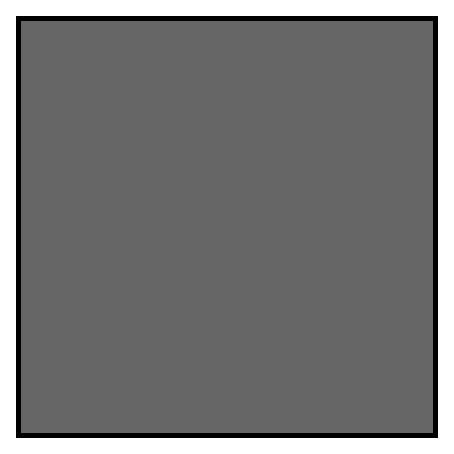
\includegraphics{example.eps}
% figure caption is below the figure
\caption{Please write your figure caption here}
\label{fig:1}       % Give a unique label
\end{figure}
%
% For two-column wide figures use
\begin{figure*}
% Use the relevant command to insert your figure file.
% For example, with the graphicx package use
  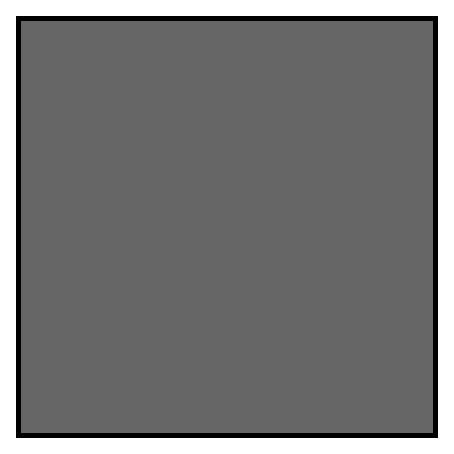
\includegraphics[width=0.75\textwidth]{example.eps}
% figure caption is below the figure
\caption{Please write your figure caption here}
\label{fig:2}       % Give a unique label
\end{figure*}
%
% For tables use
\begin{table}
% table caption is above the table
\caption{Please write your table caption here}
\label{tab:1}       % Give a unique label
% For LaTeX tables use
\begin{tabular}{lll}
\hline\noalign{\smallskip}
first & second & third  \\
\noalign{\smallskip}\hline\noalign{\smallskip}
number & number & number \\
number & number & number \\
\noalign{\smallskip}\hline
\end{tabular}
\end{table}


%\begin{acknowledgements}
%If you'd like to thank anyone, place your comments here
%and remove the percent signs.
%\end{acknowledgements}

% BibTeX users please use one of
%\bibliographystyle{spbasic}      % basic style, author-year citations
%\bibliographystyle{spmpsci}      % mathematics and physical sciences
%\bibliographystyle{spphys}       % APS-like style for physics
%\bibliography{}   % name your BibTeX data base

\bibliographystyle{spmpsci}
\bibliography{mybibtex}

\end{document}
% end of file template.tex

